Here, we derive the computation graphs for the Laplacian and its associated Gramian when using reverse-mode AD, aka backpropagation.
In contrast to the Taylor-mode perspective, the resulting expressions cannot be interpreted as simple weight-sharing.
This complicates defining a Kronecker-factored approximation for the Gramian without introducing new approximations that are different from~\citet{eschenhagen2023kroneckerfactored}, rendering the Taylor-mode perspective advantageous.

We start by deriving the Laplacian $\Delta u \coloneqq \Tr(\gradsquared{\vx} u)$ of a feed-forward NN (see \Cref{subsec:engd}), assuming a single data point for simplicity (see \Cref{sec:laplacian-computation-graph}) and abbreviating $u_{\vtheta}$ as $u$.
The goal is to make the Laplacian's dependence w.r.t.\,a weight $\mW^{(i)}$ in one layer of the network explicit.
Then, we can write down the Jacobian $\jac_{\mW^{(i)}}\Delta u$ (see \Cref{subsec:parameter-jacobian-laplacian}) which is required for the Gramian in \Cref{eq:gramian} (see \Cref{subsec-gramian-backward-laplacian}).
We do this based on the concept of \emph{Hessian backpropagation}~\citep[HBP,]{dangel2020modular} which yields a recursion for the Hessian $\gradsquared{\vx}u$.
The Laplacian follows by taking the trace of the latter.
Finally, we use the chain rule express the Laplacian's Jacobian $\jac_{\mW^{(i)}} \Delta u$ in terms of $\mW^{(i)}$'s children in the compute graph.

\subsection{Hessian Backpropagation and Backward Laplacian}\label{sec:laplacian-computation-graph}

Gradient backpropagation describes a recursive procedure to compute gradients by backpropagating a signal via vector-Jacobian products (VJPs).
A similar procedure can be derived to compute Hessians w.r.t.\,nodes in a graph ($\vz^{(i)}$ or $\vtheta^{(i)}$).
We call this recursive procedure Hessian backpropagation~\citep{dangel2020modular}.

\paragraph{Gradient backpropagation} As a warm-up, let's recall how to compute the gradient $\grad{\vtheta}u = (\grad{\vtheta^{(1)}}u, \dots, \grad{\vtheta^{(L)}}u)$.
We start by setting $\grad{\vz^{(L)}}u = \grad{u}u = 1$ (assuming $u$ is scalar for simplicity), then backpropagate the error via VJPs according to the recursion
\begin{align}\label{eq:gradient-backpropagation}
  \begin{split}
    \grad{\vz^{(i-1)}}u
    &=
      \left( \jac_{\vz^{(i-1)}} \vz^{(i)} \right)^{\top} \grad{\vz^{(i)}}u\,,
    \\
    \grad{\vtheta^{(i)}}u
    &=
      \left( \jac_{\vtheta^{(i)}} \vz^{(i)} \right)^{\top} \grad{\vz^{(i)}}u\,
  \end{split}
\end{align}
for $i = L, \dots, 1$.
This yields the gradients of $u$ w.r.t.\,all intermediate representations and parameters.

\paragraph{Hessian backpropagation} Just like gradient backpropagation, we can derive a recursive scheme for the Hessian.
Recall the Hessian chain rule
\begin{equation}\label{eq:hessianChainRule}
  \nabla^2 (f\circ g)
  =
  (\jac g)^\top \nabla^2 f(g) (\jac g)
  +
  \sum_k (\nabla_g f)_k \cdot \nabla^2 g_k,
\end{equation}
where $g_i$ denotes the individual components of $g$, see~\cite{skorski2019chain}.
The recursion for computing Hessians of $u$
w.r.t.\,intermediate representations and parameters starts by initializing the
recursion with $\gradsquared{\vz^{(L)}}u = \gradsquared{u} u = 0$, and then
backpropagating according to (see \citet{dangel2020modular} for details)
\begin{align}\label{eq:hessian-backpropagation}
  \begin{split}
    \gradsquared{\vz^{(i-1)}}u
    &=
      \left( \jac_{\vz^{(i-1)}} \vz^{(i)} \right)^{\top}
      \gradsquared{\vz^{(i)}}u
      \left( \jac_{\vz^{(i-1)}} \vz^{(i)} \right)
      +
      \sum_{k=1}^{h^{(i)}}
      \left(
      \gradsquared{\vz^{(i-1)}} [\vz^{(i)}]_k
      \right)
      [\grad{\vz^{(i)}} u]_k\,,
    \\
    \gradsquared{\vtheta^{(i)}}u
    &=
      \left( \jac_{\vtheta^{(i)}} \vz^{(i)} \right)^{\top}
      \gradsquared{\vz^{(i)}}u
      \left( \jac_{\vtheta^{(i)}} \vz^{(i)} \right)
      +
      \sum_{k=1}^{h^{(i)}}
      \left(
      \gradsquared{\vtheta^{(i)}} [\vz^{(i)}]_k
      \right)
      [\grad{\vz^{(i)}} u]_k
  \end{split}
\end{align}
for $i = L, \dots, 1$.
The first term takes the incoming Hessian (w.r.t.\,a layer's output) and sandwiches it between the layer's Jacobian.
It can be seen as backpropagating curvature from downstream layers.
The second term adds in curvature introduced by the current layer.
It is only non-zero if the layer is nonlinear.
For linear layers, convolutional layers, and ReLU layers, it is zero.

\begin{figure}[t]
  \centering
  \resizebox{\linewidth}{!}{%
    % Define styles of nodes in computation graph sketch
\tikzset{%
  % shared basic style
  basicNode/.style={%
    rectangle,%
    minimum width=5ex,%
    minimum height=3.5ex,%
    inner sep=0.3ex,%
    rounded corners,%
    draw=black,%
    thick,%
    fill opacity=0.3,%
    text opacity=1.0,%
  },%
  % style for nodes representing neural network parameters
  paramNode/.style={%
    basicNode,%
    fill=maincolor,%
  },%
  % style for nodes representing data
  inputNode/.style={%
    basicNode,%
    fill=secondcolor,%
  },%
  % style for nodes indicating a repetition
  dotsNode/.style={%
    basicNode,%
    draw opacity=0,%
  },%
  % style for nodes representing intermediates from the forward pass
  forwardNode/.style={%
    basicNode,%
    fill=thirdcolor,%
  },%
  % style for nodes representing intermediates from the gradient backpropagation
  gradientNode/.style={%
    basicNode,%
    fill=fourthcolor,%
  },%
  % style for nodes representing intermediates from the Hessian % backpropagation
  hessianNode/.style={%
    basicNode,%
    fill=fifthcolor,%
  },%
}%
%%% Local Variables:
%%% mode: latex
%%% TeX-master: "../main"
%%% End:

\begin{tikzpicture}
  % arrange nodes in a matrix
  \matrix [%
  row sep=5ex,%
  column sep=5.5ex,%
  ampersand replacement=\&,% in order to put this inside of a scalebox
  ]{%
    % neural network parameters
    \node {Parameters};
    \&
    \&
    \&
    \node [paramNode] (param-1) {$\vtheta^{(1)}$};
    \&
    \node [dotsNode] (param-2) {$\dots$};
    \&
    \node [paramNode] (param-3) {$\vtheta^{(i-1)}$};
    \&
    \node [paramNode] (param-4) {$\vtheta^{(i)}$};
    \&
    \node [dotsNode] (param-5) {$\dots$};
    \&
    \node [paramNode] (param-6) {$\vtheta^{(L)}$};
    \\
    % forward pass
    \node {Forward};
    \&
    \&
    \node [inputNode] (forward-0) {$\vx$};
    \&
    \node [forwardNode] (forward-1) {$\vz^{(1)}$};
    \&
    \node [dotsNode] (forward-2) {$\dots$};
    \&
    \node [forwardNode] (forward-3) {$\vz^{(i-1)}$};
    \&
    \node [forwardNode] (forward-4) {$\vz^{(i)}$};
    \&
    \node [dotsNode] (forward-5) {$\dots$};
    \&
    \node [forwardNode] (forward-6) {$u$};
    \\
    % gradients
    \node {Backward};
    \&
    \&
    \node [gradientNode] (gradient-0) {$\grad{\vx}u$};
    \&
    \node [gradientNode] (gradient-1) {$\grad{\vz^{(1)}}u$};
    \&
    \node [dotsNode] (gradient-2) {$\dots$};
    \&
    \node [gradientNode] (gradient-3) {$\grad{\vz^{(i-1)}}u$};
    \&
    \node [gradientNode] (gradient-4) {$\grad{\vz^{(i)}}u$};
    \&
    \node [dotsNode] (gradient-5) {$\dots$};
    \&
    \node [gradientNode] (gradient-6) {$\grad{u}u$};
    \\
    % Hessians
    \node {Hess.\,backward};
    \&
    \node [hessianNode] (laplacian) {$\Delta u$};
    \&
    \node [hessianNode] (hessian-0) {$\gradsquared{\vx}u$};
    \&
    \node [hessianNode] (hessian-1) {$\gradsquared{\vz^{(1)}}u$};
    \&
    \node [dotsNode] (hessian-2) {$\dots$};
    \&
    \node [hessianNode] (hessian-3) {$\gradsquared{\vz^{(i-1)}}u$};
    \&
    \node [hessianNode] (hessian-4) {$\gradsquared{\vz^{(i)}}u$};
    \&
    \node [dotsNode] (hessian-5) {$\dots$};
    \&
    \node [hessianNode] (hessian-6) {$\gradsquared{u}u$};
    \\
  };
  % dependency arrows
  \foreach \i in {1,...,6} {
    \draw [-Latex, thick] (param-\i) to (forward-\i);
  }
  \foreach \i in {0,...,5} {
    \draw [-Latex, thick] (forward-\i) to (gradient-\i);
    \draw [-Latex, thick] (gradient-\i) to (hessian-\i);
    \draw [-Latex, thick, out=225, in=135] (forward-\i) to (hessian-\i);
  }
  \foreach \i in {0,...,5} {
    \pgfmathsetmacro{\j}{int(\i+1)}
    \draw [-Latex, thick] (forward-\i) to (forward-\j);
    \draw [-Latex, thick] (gradient-\j) to (gradient-\i);
    \draw [-Latex, thick] (hessian-\j) to (hessian-\i);
  }
  \foreach \i in {0,...,5} {
    \pgfmathsetmacro{\j}{int(\i+1)}
    \draw [-Latex, thick, out=215, in=45] (param-\j) to (gradient-\i);
    \draw [-Latex, thick, out=235, in=45] (param-\j) to (hessian-\i);
  }
  \draw [-Latex, thick] (hessian-0) to (laplacian);
\end{tikzpicture}
%%% Local Variables:
%%% mode: latex
%%% TeX-master: "../main"
%%% End:

  }
  \caption{Computation graph of a sequential neural network's Laplacian $\Delta u$ when using (Hessian) backpropagation.
    Arrows indicate dependencies between intermediates.
    Note that $\vz^{(0)} \coloneqq \vx$, $\vz^{(L)} \coloneqq u$, $\grad{u}u = 1$, and $\gradsquared{u}u = \vzero$.
    For the Gramian, we are interested in how the neural network parameters enter the Laplacian's computation. Each parameter is used three times: during (i) the forward pass, (ii) the backward pass for the gradient, and (iii) the backward pass for the Hessian.}\label{fig:hbp-dependencies}
\end{figure}

Following the Hessian backpropagation procedure of \Cref{eq:hessian-backpropagation} yields the
per-layer parameter and feature Hessians $\gradsquared{\vz^{(i)}}u,
\gradsquared{\vtheta^{(i)}}u$. In \Cref{fig:hbp-dependencies} we depict the dependencies of
intermediate gradients and Hessians for computing $\gradsquared{\vx}u = \gradsquared{\vz^{(0)}}u$:
\begin{itemize}
\item $\grad{\vz^{(i-1)}}u$ depends on $\grad{\vz^{(i)}}u$ due to the recursion in \Cref{eq:gradient-backpropagation}, and on $\vz^{(i-1)}, \vtheta^{(i)}$ due to the Jacobian $\mJ_{\vz^{(i-1)}}\vz^{(i)}$ in the gradient backpropagation \Cref{eq:gradient-backpropagation}.

\item $\gradsquared{\vz^{(i-1)}}u$ depends on $\gradsquared{\vz^{(i)}}u$ and $\grad{\vz^{(i)}} u$ due to the recursion in \Cref{eq:hessian-backpropagation}, and on $\vz^{(i-1)}, \vtheta^{(i)}$ due to the Jacobian $\mJ_{\vz^{(i-1)}}\vz^{(i)}$ and Hessian $\gradsquared{\vz^{(i-1)}}[\vz^{(i)}]_k$ in the Hessian backpropagation \Cref{eq:gradient-backpropagation}.
\end{itemize}

The Laplacian $\Delta u$ follows by taking the trace of
$\gradsquared{\vx}u$ from above, and is hence recursively defined.
To make these expressions more concrete, we now recap the HBP equations for fully-connected layers and element-wise nonlinear activations.


\paragraph{Hessian backpropagation through nonlinear layers}
We mostly consider nonlinear layers without trainable parameters and consist of a componentwise nonlinearity $z\mapsto \sigma(z)$ for some $\sigma\colon\mathbb R\to\mathbb R$.
The Jacobian of such a nonlinear layer is given by $\jac_{\vz^{(i-1)}}\vz^{(i)} = \diag(\sigma'(\vz^{(i-1)}))$ and the Hessian terms are given by $\nabla^2_{\vz^{(i-1)}}[\vz^{(i)}]_k = \sigma''(\vz^{(i-1)}_k) \ve_k \ve_k^\top$ where $\ve_k$ is the unit vector along coordinate $k$.
With these two identities we can backpropogate the input Hessian through such layers via
\begin{align}
  \begin{split}
    \gradsquared{\vz^{(i-1)}}u
    &=
      \left( \diag(\sigma'(\vz^{(i-1)})) \right)^{\top}
      \gradsquared{\vz^{(i)}}u
      \left( \diag(\sigma'(\vz^{(i-1)})) \right)
    \\
    &\phantom{=}+
      \sum_{k=1}^{h^{(i)}}
      \sigma''(\vz^{(i-1)}_k)
      \ve_k \ve_k^\top
      [\grad{\vz^{(i)}} u]_k\,.
  \end{split}
\end{align}

\paragraph{Hessian backpropagation through a linear layer} To de-clutter the dependency graph of \Cref{fig:hbp-dependencies}, we will now consider the dependency of $\Delta u$ w.r.t.\,the weight of a single layer.
We assume this layer $i$ to be a linear layer with parameters $\mW^{(i)}$ such that $\vtheta^{(i)} = \flatten(\mW^{(i)})$,
\begin{align}
  \vz^{(i)} = \mW^{(i)} \vz^{(i-1)}\,.
\end{align}
For this layer, the second terms in \Cref{eq:hessian-backpropagation} disappears because the local Hessians are zero, that is $\gradsquared{\vz^{(i-1)}}[\vz^{(i)}]_k = \vzero$ and $\gradsquared{\mW^{(i)}}[\vz^{(i)}]_k = \vzero$.
Also, the Jacobians are $\jac_{\mW^{(i)}}\vz^{(i)} = {\vz^{(i-1)}}^{\top} \otimes \mI$ and $\jac_{\vz^{(i-1)}}\vz^{(i)} = \mW^{(i)}$ and hence only depend on one of the two layer inputs.
This simplifies the computation graph.
\Cref{fig:laplacian-graph-weight} shows the dependencies of $\mW^{(i)}$ on the
Laplacian, highlighting its three direct children,
\begin{align}\label{eq:spatialDerivatives}
  \begin{split}
    \vz^{(i)}
    &=
      \mW^{(i)} \vz^{(i-1)}\,,
    \\
    \grad{\vz^{(i-1)}}u
    &=
      {\mW^{(i)}}^{\top}
      \left(
      \grad{\vz^{(i)}}u
      \right)\,,
    \\
    \gradsquared{\vz^{(i-1)}}u
    &=
      {\mW^{(i)}}^{\top}
      \left(
      \gradsquared{\vz^{(i)}}u
      \right)
      \mW^{(i)}\,.
  \end{split}
\end{align}

\begin{figure}[t]
  \centering
  \begin{minipage}[b]{0.495\linewidth}
    \centering
    \resizebox{\linewidth}{!}{%
      % Define styles of nodes in computation graph sketch
\tikzset{%
  % shared basic style
  basicNode/.style={%
    rectangle,%
    minimum width=5ex,%
    minimum height=3.5ex,%
    inner sep=0.3ex,%
    rounded corners,%
    draw=black,%
    thick,%
    fill opacity=0.3,%
    text opacity=1.0,%
  },%
  % style for nodes representing neural network parameters
  paramNode/.style={%
    basicNode,%
    fill=maincolor,%
  },%
  % style for nodes representing data
  inputNode/.style={%
    basicNode,%
    fill=secondcolor,%
  },%
  % style for nodes indicating a repetition
  dotsNode/.style={%
    basicNode,%
    draw opacity=0,%
  },%
  % style for nodes representing intermediates from the forward pass
  forwardNode/.style={%
    basicNode,%
    fill=thirdcolor,%
  },%
  % style for nodes representing intermediates from the gradient backpropagation
  gradientNode/.style={%
    basicNode,%
    fill=fourthcolor,%
  },%
  % style for nodes representing intermediates from the Hessian % backpropagation
  hessianNode/.style={%
    basicNode,%
    fill=fifthcolor,%
  },%
}%
%%% Local Variables:
%%% mode: latex
%%% TeX-master: "../main"
%%% End:

\begin{tikzpicture}
  % arrange nodes in a matrix
  \matrix [%
  row sep=5ex,%
  column sep=5.5ex,%
  ampersand replacement=\&,% in order to put this inside of a scalebox
  ]{%
    % neural network parameters
    \&
    \&
    \node [dotsNode] (param-1) {$\dots$};
    \&
    \node [paramNode] (weight) {$\mW^{(i)}$};
    % \node [paramNode, anchor=west, xshift=0.5ex] (bias) at (weight.east) {$\vb^{(i)}$};
    \&
    \node [dotsNode] (param-3) {$\dots$};
    \\
    % forward pass
    \&
    \node [dotsNode] (forward-1) {$\dots$};
    \&
    \node [forwardNode] (forward-2) {$\vz^{(i-1)}$};
    \&
    \node [forwardNode] (forward-3) {$\vz^{(i)}$};
    \&
    \node [dotsNode] (forward-4) {$\dots$};
    \\
    % gradients
    \&
    \node [dotsNode] (gradient-1) {$\dots$};
    \&
    \node [gradientNode] (gradient-2) {$\grad{\vz^{(i-1)}}u$};
    \&
    \node [gradientNode] (gradient-3) {$\grad{\vz^{(i)}}u$};
    \&
    \node [dotsNode] (gradient-4) {$\dots$};
    \\
    % Hessians
    \node [hessianNode] (laplacian) {$\Delta u$};
    \&
    \node [dotsNode] (hessian-1) {$\dots$};
    \&
    \node [hessianNode] (hessian-2) {$\gradsquared{\vz^{(i-1)}}u$};
    \&
    \node [hessianNode] (hessian-3) {$\gradsquared{\vz^{(i)}}u$};
    \&
    \node [dotsNode] (hessian-4) {$\dots$};
    \\
  };
  % dependency arrows
  \foreach \i in {1,3} {
    \pgfmathsetmacro{\j}{int(\i+1)}
    \draw [-Latex, thick] (param-\i) to (forward-\j);
  }
  \foreach \i in {1,...,4} {
    \draw [-Latex, thick] (forward-\i) to (gradient-\i);
    \draw [-Latex, thick] (gradient-\i) to (hessian-\i);
    \draw [-Latex, thick, out=225, in=135] (forward-\i) to (hessian-\i);
  }
  \foreach \i in {1,...,3} {
    \pgfmathsetmacro{\j}{int(\i+1)}
    \draw [-Latex, thick] (forward-\i) to (forward-\j);
    \draw [-Latex, thick] (gradient-\j) to (gradient-\i);
    \draw [-Latex, thick] (hessian-\j) to (hessian-\i);
  }
  \foreach \i in {1,3} {
    \pgfmathsetmacro{\j}{int(\i)}
    \draw [-Latex, thick, out=215, in=45] (param-\i) to (gradient-\j);
    \draw [-Latex, thick, out=235, in=45] (param-\j) to (hessian-\j);
  }
  \draw [-Latex, thick] (hessian-1) to (laplacian);
  \draw [-Latex, ultra thick, secondcolor] (weight) to (forward-3);
  \draw [-Latex, ultra thick, secondcolor, out=215, in=45] (weight) to (gradient-2);
  \draw [-Latex, ultra thick, secondcolor, out=235, in=45] (weight) to (hessian-2);
\end{tikzpicture}
%%% Local Variables:
%%% mode: latex
%%% TeX-master: "../main"
%%% End:

    }
  \end{minipage}
  \hfill
  \begin{minipage}[b]{0.495\linewidth}
    \caption{Direct dependencies of a linear layer's weight matrix $\mW^{(i)}$ in the Laplacian's computation graph.
      There are three direct children: (i) the layer's output from the forward pass, (ii) the Laplacian's gradient w.r.t.\,the layer's input from the gradient backpropagation, and (iii) the Laplacian's Hessian w.r.t.\,the layer's input from the Hessian backpropagation.
      The Jacobians $\jac_{\mW^{(i)}}\Delta u$ required for the Gramian are the vector-Jacobian products accumulated over those children.
    }\label{fig:laplacian-graph-weight}
    \vspace{-1ex}
  \end{minipage}
\end{figure}

\subsection{Parameter Jacobian of the Backward Laplacian}\label{subsec:parameter-jacobian-laplacian}
Recall that the entries of the Gramian are composed from parameter derivatives of the input Laplacian, see~\Cref{eq:gramian}.
We have identified the direct children of $\mW^{(i)}$ in the Laplacian's compute graph, see \Cref{eq:spatialDerivatives}.
This allows us to compute the Jacobian $\jac_{\mW^{(i)}} \Delta u$ by the chain rule, i.e.\,by accumulating the Jacobians over all direct children,
\begin{align}\label{eq:laplacian-gradient}
  \begin{split}
    \jac_{\mW^{(i)}} \Delta u
    &=
      \textstyle
      \sum_{\bullet \in \left\{ \vz^{(i)}, \grad{\vz^{(i-1)}}u, \gradsquared{\vz^{(i-1)}}u \right\}}
      \left(
      \jac_{\mW^{(i)}}\bullet
      \right)^{\top}
      \grad{\bullet}\Delta u
    \\
    &=
      \left(
      \jac_{\mW^{(i)}}\vz^{(i)}
      \right)^{\top}
      \grad{\vz^{(i)}}\Delta u
    \\
    &\phantom{=}+
      \left(
      \jac_{\mW^{(i)}}\grad{\vz^{(i-1)}}u
      \right)^{\top}
      \grad{\grad{\vz^{(i-1)}}u}\Delta u
    \\
    &\phantom{=}+
      \left(
      \jac_{\mW^{(i)}}\gradsquared{\vz^{(i-1)}}u
      \right)^{\top}
      \grad{\gradsquared{\vz^{(i-1)}}u}\Delta u\,.
  \end{split}
\end{align}
The terms $\grad{\bullet}\Delta u$ can be computed with gradient backpropagation to the respective intermediates.

\subsection{Gramian of the Backward Laplacian}\label{subsec-gramian-backward-laplacian}

With the Laplacian's Jacobian from \Cref{eq:laplacian-gradient}, we can now write down the Gramian block of the interior loss (up to summation over the data) for $\mW^{(i)}$ as
\begin{align}\label{eq:fisher}
  \begin{split}
    \mG_{\Omega}^{(i)}
    &=
      \left(
      \jac_{\mW^{(i)}} \Delta u
      \right)
      \left(
      \jac_{\mW^{(i)}} \Delta u
      \right)^{\top}
    \\
    &=
      \textstyle
      \sum_{\textcolor{blue}{\bullet}, \textcolor{red}{\bullet} \in \left\{ \vz^{(i)}, \grad{\vz^{(i-1)}}u, \gradsquared{\vz^{(i-1)}}u \right\}}
      \underbrace{
      \left(
      \jac_{\mW^{(i)}}\textcolor{blue}{\bullet}
      \right)^{\top}
      \left[
      \left(
      \grad{\textcolor{blue}{\bullet}}\Delta u
      \right)
      \left(
      \grad{\textcolor{red}{\bullet}}\Delta u
      \right)^{\top}
      \right]
      \left(
      \jac_{\mW^{(i)}}\textcolor{red}{\bullet}
      \right)}_{
      \eqqcolon \mG_{\Omega,\textcolor{blue}{\bullet}, \textcolor{red}{\bullet}}^{(i)}
      }\,.
  \end{split}
\end{align}
The Gramian consists of nine different terms, see \Cref{fig:gramian-contribution-children} for a visualization which shows not only the diagonal blocks $\mG_{\Omega}^{(i)}$, but also the full Gramian $\mG_{\Omega}$ which decomposes in the same way.
The terms $\grad{\textcolor{blue}{\bullet}}\Delta u$ are automatically computed when computing the gradient of the loss via backpropagation.
We will now proceed and simplify the terms by inserting the Jacobians into \Cref{eq:laplacian-gradient} and studying the Gramian's block diagonal, which is approximated by KFAC, in more detail.

\begin{figure}[t]
  \centering
  Full interior Gramian\\
  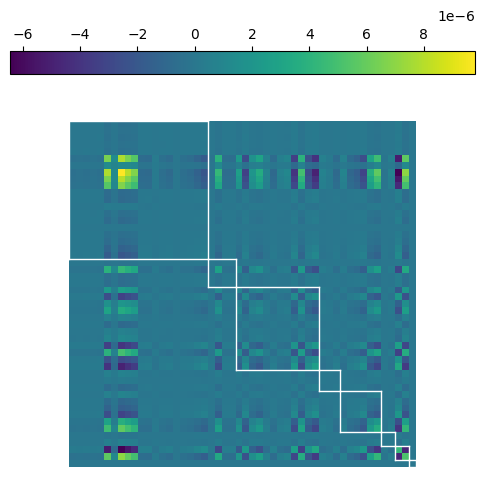
\includegraphics[width=0.43\linewidth]{kfac_pinns_exp/exp04_gramian_contributions/fig/gram_full.png}

  \begin{tabular}{ccc}
    (\textcolor{blue}{forward}, \textcolor{red}{forward})
    &
      (\textcolor{blue}{forward}, \textcolor{red}{gradient})
    &
      (\textcolor{blue}{forward}, \textcolor{red}{Hessian})
    \\
    
\includegraphics[width=0.22\linewidth]{kfac_pinns_exp/exp04_gramian_contributions/fig/gram_output_output.png}
    &
      
\includegraphics[width=0.22\linewidth]{kfac_pinns_exp/exp04_gramian_contributions/fig/gram_output_grad_input.png}
    &
      
\includegraphics[width=0.22\linewidth]{kfac_pinns_exp/exp04_gramian_contributions/fig/gram_output_hess_input.png}
    \\
    (\textcolor{blue}{gradient}, \textcolor{red}{forward})
    &
      (\textcolor{blue}{gradient}, \textcolor{red}{gradient})
    &
      (\textcolor{blue}{gradient}, \textcolor{red}{Hessian})
    \\
    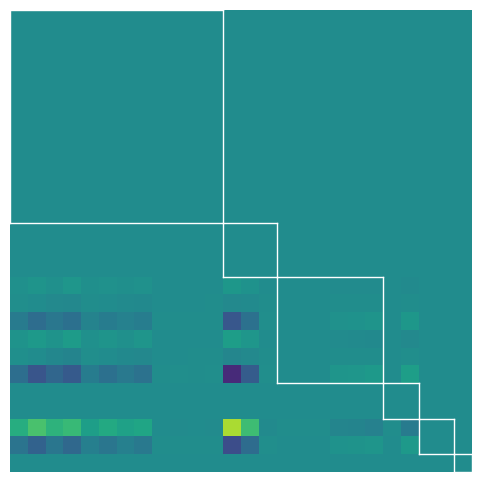
\includegraphics[width=0.22\linewidth]{kfac_pinns_exp/exp04_gramian_contributions/fig/gram_grad_input_output.png}
    &
      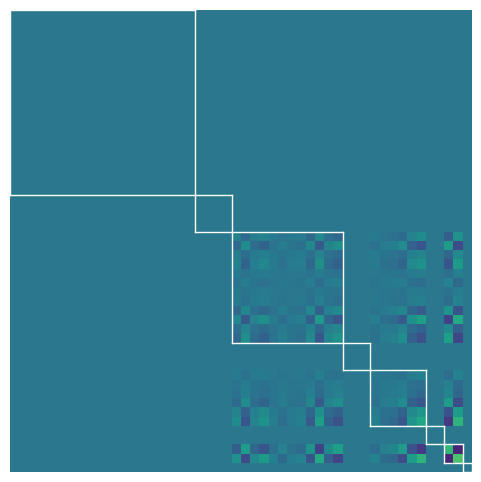
\includegraphics[width=0.22\linewidth]{kfac_pinns_exp/exp04_gramian_contributions/fig/gram_grad_input_grad_input.png}
    &
      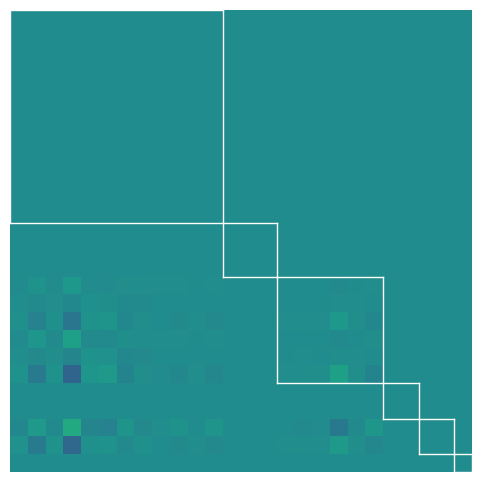
\includegraphics[width=0.22\linewidth]{kfac_pinns_exp/exp04_gramian_contributions/fig/gram_grad_input_hess_input.png}
    \\
    (\textcolor{blue}{Hessian}, \textcolor{red}{forward})
    &
      (\textcolor{blue}{Hessian}, \textcolor{red}{gradient})
    &
      (\textcolor{blue}{Hessian}, \textcolor{red}{Hessian})
    \\
    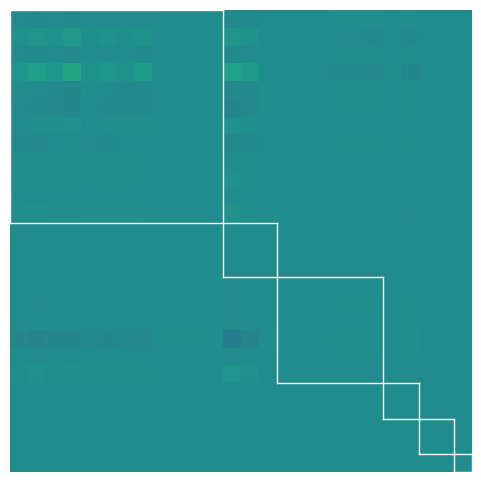
\includegraphics[width=0.22\linewidth]{kfac_pinns_exp/exp04_gramian_contributions/fig/gram_hess_input_output.png}
    &
      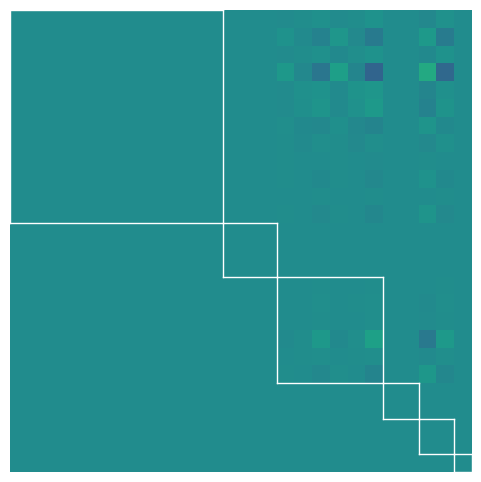
\includegraphics[width=0.22\linewidth]{kfac_pinns_exp/exp04_gramian_contributions/fig/gram_hess_input_grad_input.png}
    &
      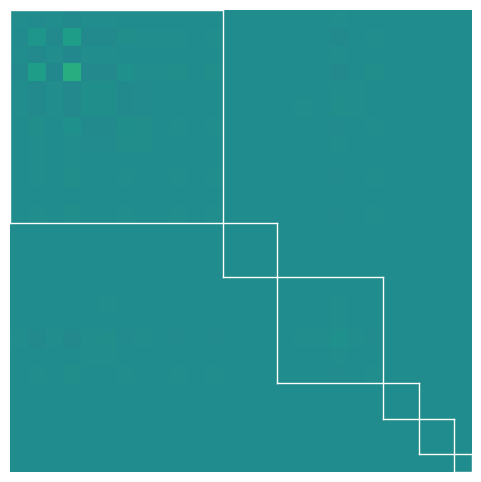
\includegraphics[width=0.22\linewidth]{kfac_pinns_exp/exp04_gramian_contributions/fig/gram_hess_input_hess_input.png}
  \end{tabular}
  \caption{Contributions $\mG_{\Omega,\textcolor{blue}{\bullet}, \textcolor{red}{\bullet}}$ to the Laplacian's Gramian $\mG_{\Omega}$ from different children in the computation graph on a synthetic toy problem.
    We use a $4 \to 3 \to 2 \to 1$ sigmoid-activated MLP and 10 randomly generated inputs. The contributions are highlighted as in \Cref{eq:fisher}.}\label{fig:gramian-contribution-children}
\end{figure}
%%% Local Variables:
%%% mode: latex
%%% TeX-master: "../main"
%%% End:


\paragraph{Computing $\jac_{\mW^{(i)}}\bullet$}
Let us first compute the Jacobians $\jac_{\mW^{(i)}}\bullet$ in \Cref{eq:laplacian-gradient}.
The Jacobian of the linear layer's forward pass is
\begin{subequations}\label{eq:fisher-jacobians}
  \begin{align}
    \jac_{\mW}\left( \mW \vx \right) = \vx^{\top} \otimes \mI\,.
  \end{align}
  The Jacobian from the gradient backpropagation is
  \begin{align}
    \jac_{\mW}\left( \mW^{\top} \vx \right) = \mI \otimes \vx^{\top}\,,
  \end{align}
  and the Jacobian from the Hessian backpropagation is
  \begin{align}\label{subeq:fisher-jacobians-hbp}
    \jac_{\mW}\left( \mW^{\top} \mX \mW \right)
    =
    \mI \otimes \mW^{\top}\mX
    +
    \mK \left(
    \mI
    \otimes
    \mW^{\top}\mX^{\top}
    \right)\,,
  \end{align}
\end{subequations}
where $\mK \in \sR^{\dim(\mZ) \times \dim(\mZ)}$ (denoting $\mZ := \mW^{\top}\mX \mW$) is a permutation matrix that, when multiplied onto a vector whose basis corresponds to that of the flattened output $\mZ$, modifies the order from first-varies-fastest to last-varies-fastest, i.e.
\begin{equation*}
  \mK \flatten(\mZ) = \flatten(\mZ^{\top})\,.
\end{equation*}
Re-introducing the layer indices, the expressions in \Cref{eq:spatialDerivatives} become
\begin{align}
  \begin{split}
    \jac_{\mW^{(i)}}\vz^{(i)}
    &=
      {\vz^{(i-1)}}^\top\otimes \mI
    \\
    \jac_{\mW^{(i)}}\grad{\vz^{(i-1)}}u\,,
    &=
      \mI\otimes
      \grad{\vz^{(i)}}u
    \\
    \jac_{\mW^{(i)}}\gradsquared{\vz^{(i-1)}}u\,,
    &=
      \mI \otimes
      \left[
      {\mW^{(i)}}^{\top}
      \left(
      \gradsquared{\vz^{(i)}}u
      \right)
      \right]
      +
      \mK
      \left(
      \mI \otimes
      \left[
      {\mW^{(i)}}^{\top}
      \left(
      \gradsquared{\vz^{(i)}}u
      \right)^{\top}
      \right]
      \right)\,.
  \end{split}
\end{align}
We will now use symmetries in the objects used during Hessian backpropagation to simplify this further.
At a first glance, it looks like the Gramian consists of 16 terms, as there are 4 summands from the Jacobians in \Cref{eq:fisher-jacobians}.
However, we can simplify into 9 terms:

First, $\gradsquared{\vz^{(i)}}u$ is symmetric, that is
\begin{align*}
  \jac_{\mW^{(i)}}\left( {\mW^{(i)}}^{\top} \left( \gradsquared{\vz^{(i)}}u  \right)\mW^{(i)} \right)
  &=
    \mI \otimes
    \left[
    {\mW^{(i)}}^{\top} \left( \gradsquared{\vz^{(i)}}u  \right)
    \right]
    +
    \mK
    \left(
    \mI \otimes
    \left[
    {\mW^{(i)}}^{\top}
    \left(
    \gradsquared{\vz^{(i)}}u
    \right)
    \right]
    \right)\,,
    \shortintertext{and the transposed Jacobian is}
  &\mI \otimes
    \left[
    \left( \gradsquared{\vz^{(i)}}u  \right) \mW^{(i)}
    \right]
    +
    \left(
    \mI \otimes
    \left[
    \left(
    \gradsquared{\vz^{(i)}}u
    \right)
    \mW^{(i)}
    \right]
    \right)
    \mK^{\top}\,.
\end{align*}
Second, we multiply the transpose Jacobian onto $\grad{\gradsquared{\vz^{(i-1)}}u}\Delta u$, which inherits symmetry from the Hessian, $[\grad{\gradsquared{\vz^{(i-1)}}u}\Delta u]_{j,k} = [\grad{\gradsquared{\vz^{(i-1)}}u}\Delta u]_{k,j}$.
Due to this symmetry, the action of $\mK$ (or $\mK^{\top}$) does not alter it,
\begin{align*}
  \mK^{\top}\left( \grad{\gradsquared{\vz^{(i-1)}}u}\Delta u \right) = \grad{\gradsquared{\vz^{(i-1)}}u}\Delta u\,.
\end{align*}
In other words, it does not matter how we flatten (first- or last-varies-fastest).
This simplifies the VJP (last line in \Cref{eq:fisher}) to
\begin{align*}
  \left(
  \mI \otimes
  \left[
  \left( \gradsquared{\vz^{(i)}}u  \right) \mW^{(i)}
  \right]
  \right)
  \grad{\gradsquared{\vz^{(i-1)}}u}\Delta u
  +
  \left(
  \mI \otimes
  \left[
  \left(
  \gradsquared{\vz^{(i)}}u
  \right)
  \mW^{(i)}
  \right]
  \right)
  \mK^{\top}
  \grad{\gradsquared{\vz^{(i-1)}}u}\Delta u
  \\
  =
  2 \left(
  \mI \otimes
  \left[
  \left( \gradsquared{\vz^{(i)}}u  \right) \mW^{(i)}
  \right]
  \right)
  \grad{\gradsquared{\vz^{(i-1)}}u}\Delta u
  \,.
\end{align*}
We can now write down the simplified Jacobian from \Cref{eq:laplacian-gradient}, whose self-outer product forms the Gramian block for a linear layer's weight matrix,
\begin{align}\label{eq:weight-jacobian-simplified}
  \begin{split}
    \jac_{\mW^{(i)}} \Delta u
    &=
      \underbrace{
      \left(
      {\vz^{(i-1)}}^\top\otimes \mI
      \right)^{\top}
      \grad{\vz^{(i)}}\Delta u
      }_{(1)}
    \\
    &\phantom{=}+
      \underbrace{
      \left(
      \mI \otimes \grad{\vz^{(i)}}u
      \right)^{\top}
      \grad{\grad{\vz^{(i-1)}}u}\Delta u
      }_{(2)}
    \\
    &\phantom{=}+
      \underbrace{
      2
      \left(
      \mI \otimes
      \left[
      \left( \gradsquared{\vz^{(i)}}u \right) \mW^{(i)}
      \right]
      \right)
      \grad{\gradsquared{\vz^{(i-1)}}u}\Delta u
      }_{(3)}
      \,,
  \end{split}
\end{align}
where (1) is the contribution from the forward pass, (2) is the contribution from the gradient backpropagation, and (3) is the contribution from the Hessian backpropagation. The Jacobians from \Cref{eq:fisher-jacobians} allow to express the Gramian in terms of Kronecker-structured expressions consisting of 9 terms in total. \Cref{fig:gramian-contribution-children} shows the 6 contributions from different children pairs.

\paragraph{Conclusion} One problem of computing the Laplacian and its Jacobian with backpropagation according to \Cref{eq:weight-jacobian-simplified} is that if we write out the Gramian's block $\mG_{\Omega}^{(i)} = \jac_{\mW^{(i)}} \Delta u (\jac_{\mW^{(i)}} \Delta u)^{\top}$, we obtain 9 terms of different structure.
Defining a single Kronecker product approximation would involve introducing new approximations on top of those employed by \citet{eschenhagen2023kroneckerfactored}.
Therefore, the forward Laplacian, or Taylor-mode, perspective we choose in the main text is advantageous as it allows to define KFAC without introducing new approximations.


%%% Local Variables:
%%% mode: latex
%%% TeX-master: "../main"
%%% End:
